\section{A photo trip to Sic Semper Tyrannis}
    \begin{marginfigure}
        \begin{tikzpicture}
            \node [name-dest] (box){%
                \begin{minipage}{0.80\textwidth}
                    \begin{itemize}
                        \item Rhys Tyers
                        \item Tanguy Racine
                    \end{itemize}
                \end{minipage}
            };
            \node[fancytitle, right=10pt] at (box.north west) {At World's End};
        \end{tikzpicture}
    \end{marginfigure}

    The breeze made the leaves rustle, their shadows dancing on the smooth, white carbonate sand. The air was cooler by the \passage[river]{So\v{c}a} river, and the sound of merry children splashing about in their inflatable dinghies upstream was a welcome change from the bivi conversations. 
    After the desolation of the windswept, grey skies of the plateau, I thought it was time to come back down in the valley and enjoy the grapefruit beers and meaty pizze. The sun was a nice addition too, so Jarv drove a team of us to Most Na Soci, where the Idrija river joined the Soca. The beers were left in the cold water while I blew air into side compartments the boat. 
    I enjoyed then a few rides on the river, mainly trying to enforce coordination in the paddling, which enabled Rhys and I to turn the boat round and maintain our position with synchronised movements, prow against the current. The beauty and complexity of the manoeuvre was lost on the bystanders unfortunately so we ran her aground lower downstream and carried the boat back to the take off. Then I sat on my towel and enjoyed the sight.

    \begin{figure*}[b!]
        \begin{tikzpicture}
        \node [name-dest] (box){%
            \begin{minipage}{\textwidth}
                \begin{parcolumns}{2}
                    \emph{In the meantime, far underground...}

                    Booze, dope, woman. Such a perfect day.
                    After that endless 230m of passage we bolted a traverse across a pitch (not pushed, too wet), we found another 20m of that passage which ended in a ... hmmm ... prelom? Full of water. It continues in the same direction (N-> S) on at least two levels. We pushed some 50m but stopped before
                    23
                    a small pitch because we left the gear behind. There you can hear water around the corner. We returned to the gear in the big “prelom” and followed the water. We made a descent (cc 30m) turned back south and squeezed through a needle hole and came to a big pitch (30m+). We could not see the bottom. We only had 15m of rope which we left on an anchor. Then we turned back and lived happily ever after.
                    O, jeah [sic] ... no surveying today. At least 5 times more water than yesterday !! Still we would like the last pitch we found to be named ‘Time to say Goodbye”.

                    Tja\v{s}a 14:30
                    In life we must do only one thing: die. So, who the hell came up with caving?
                    \name{Grega Maffi}
                \end{parcolumns}
            \end{minipage}};
        \node[fancytitle, right=10pt] at (box.north west) {Logbook extracts: Andrea Bocelli};
        \end{tikzpicture}
    \end{figure*}


    After a moment I spoke with Rhys. 
    'There are very few photos of the southern extensions of the system' he remarked, lifting his eyebrow.  That was true. 'You intend to take some?' 
    'Probably.. Yes'. 
    'How was the pushing with Ben' How about the pitch you found' Does it go?' I replied.
    'We followed the water from Sic Semper Tyrannis, and stopped at a pitch...yes, that would be a good trip wouldn't it?'
    'Yes, go down, photograph then push. I'm interested in this business of taking photos of Helm's Deep chamber and the rest, it could be impressive'
    'sure, RT and TR again''
    'Count me in!' I said, looking at the colourful valley. On the morrow, we bid farewell to Tolmin and ascended to the plateau once again. The weather turned, temperatures rose, and the sun came out as Rhys and I prepared our kit.
    \sidenote{Editor's note: This is only the author's reproduction of a half-forgotten conversation. Rhys Tyers doesn't actually use this syntax in speech.}

    Two days later, we were descending to \passage{X-Ray} with a good plan, three nights, two pushing trips. The first would be to \passage{Atlantis} and its extensions, to document the finds from the last three years with photographs. 

    We started the session at the \passage{Red Baron} chamber traverse, and worked our way to \passage{Stuck in Paradise}. After the pitch, some quick photographs of the \passage{Atlantis} stalactites saw us reach \passage{Helm's Deep} chamber. A rope led up to \passage{Touching the Void}, at the top of a loose rubble slope, underneath a fallen slab of white limestone. Ascending up there I gained a good view of the chamber some 20 metre higher than Rhys. I slid underneath the slab and carried on climbing, until I popped out onto a pitch head. Water from two streams could be seen joining into a waterfall, and a climb up led to another vantage point overlooking the pitch. The top of the pitch was again a loose slope, disappearing into the darkness above. A lead for bolt climbers which could be reached by traversing over the rock bridge I stood on, then over the drop, and further up still for another 15m. 

    The sight of the water however reminded us that exploration needs to be thorough, as well as exciting. Caver legends such as Norbert Casteret were, after all, hydrogeologists as well as speleologists. Where did that water go' Where did it come from' The former question was more easily answered, so we climbed down to the bottom of \passage{Helm's Deep} chamber, where an opening in the slope led to a water chamber of modest dimensions.

    \begin{figure*}[t!]
        \checkoddpage \ifoddpage \forcerectofloat \else \forceversofloat \fi
        \centering
        \begin{subfigure}[t]{0.68\textwidth}
            \centering
            \frame{\includegraphics[width=\linewidth]{"images/2015/tanguy-photography-2015/belowhelm_sdeep".jpg}}
            \caption{}\label{water chamber below helm's deep}
        \end{subfigure}
        \hfill
        \begin{subfigure}[t]{0.303\textwidth}
            \centering
            \frame{\includegraphics[width=\linewidth]{"images/2015/tanguy-photography-2015/rhystyers_sic_semper__1_".jpg}}
            \caption{} \label{HelmsDeep}
        \end{subfigure}

        \vspace{0.3cm}
        
        \begin{subfigure}[t]{\textwidth}
            \centering
            \frame{\includegraphics[width=\linewidth]{"images/2015/tanguy-photography-2015/rhystyers_touching_the_void__1_".jpg}} 
            \caption{} \label{Touching the Void 1}
        \end{subfigure}
        
        \caption{
            \emph{a} Water chamber below \protect\passage{Helm's Deep}
            \emph{b} In \protect\passage{Helm's Deep} chamber
            \emph{c} The top of the climb in \protect\passage{Touching the Void}, where a 30m pitch takes in the active waterfall --- Rhys Tyers 
        }
    \end{figure*}

    A small stream emerged from an obscure fissure which enlarged to an anthropic opening on top. Rhys climbed up into the rift a metre above the water and followed the passage leading off upstream. At every meander, sharp prongs of rock remained, catching on our suits, forcing us to negotiate the climb with care. A few twists and turns followed, until a flat out, damp crawl connected with the base of a large pitch. The rumble of the water rushing down resonated all around, and a slight drizzle dusted Rhys's shoulders with glittering droplets. This was the bottom of the two-waterfall pitch, underneath the pile of  cave sediment that make the floor of \passage{Helm's Deep} chamber. 

    \begin{figure*}[t!]
        \checkoddpage \ifoddpage \forcerectofloat \else \forceversofloat \fi
        \centering
        \frame{\includegraphics[width=\linewidth]{"images/2015/tanguy-photography-2015/helmsdeep".jpg}} 

        \caption{An extended elevation view of \protect\passage{Helm's Deep} chamber and adjoining \protect\passage{Touching the Void} extensions ---scanned from 2015 underground logbook}
        \label{helms deep}
         
    \end{figure*}

    The first piece of the puzzle fell into place. Back at the water chamber, we could see the stream disappearing into a tube. This almost certainly leads to the lower water chamber which is the termination of \passage{Sic Semper Tyrannis}. In the latter, the water flows underneath boulders to \passage{Davy Jones' Locker} passage. Swiftly, we caved towards the pushing front, trying to piece together the hydrology of this region of cave. Following the water, past the sump bypass flat out crawl, to the undescended pitch Rhys and Ben had found earlier. At the head, I put in a bolt, backed-up by two sling anchors and tied up a Y-hang knot. When I looked at the remaining length of rope available to descend, I let out a loud curse. Either rope we'd brought was too short on its own after the knots were tied. 

    \begin{figure*}[h]
        \checkoddpage \ifoddpage \forcerectofloat \else \forceversofloat \fi
        \centering
        \frame{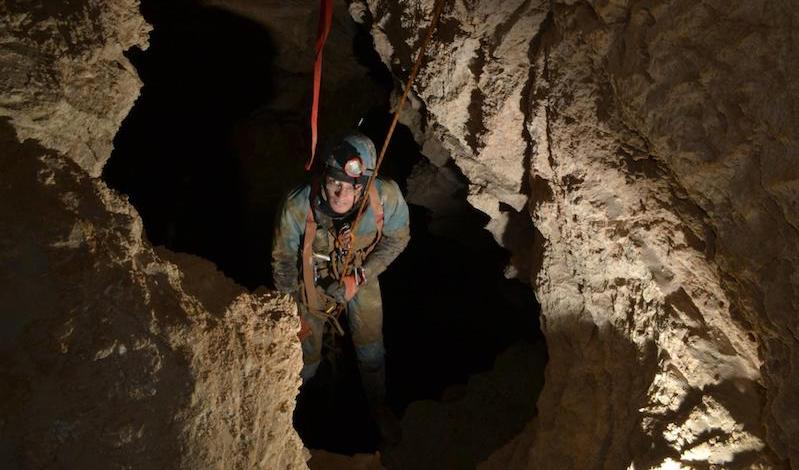
\includegraphics[width=\textwidth]{images/2015/tanguy-photography-2015/worldsend2015.jpg}}
        
        \caption{The fossil pitch named '\protect\passage{At Worlds End}' which is found downstream of the \protect\passage{Sic Semper Tyrannis} waterfall --- Rhys Tyers}
        \label{water chamber below helm's deep}
    \end{figure*}

    I had learned how tie two ropes together beforehand' whether I'd trust my life with it was another matter. After a few minutes deliberating however, we'd satisfied ourselves that if it had been done to descend '\passage{Godzilla}', with not one, or two, but three knots, then surely it could be done again. Not that our own pitch was such a monster, but soon after the take off, the pitch belled out, and after the knot pass, a smooth descent brought me on top of a boulder pile, in a dry chamber. Rhys came down soon after. There was no obvious way on, though the rumble of water could be heard, so we searched for man sized openings between the carefully positioned boulders. Dropping down a few metres brought us to a tight rift, heading west. 10 metres farther, the rift opened onto a small balcony overlooking a sizeable pitch, where the sound from a cascading streamway could be heard. To our left, the spray from the \passage{Davy Jones' Locker} almost reached us, while to the right, the morphology of the pitch suggested a far larger inlet of water down below. 

    \begin{figure*}[t!]
        \checkoddpage \ifoddpage \forcerectofloat \else \forceversofloat \fi
        \centering
        \begin{subfigure}[t]{0.41\textwidth}
            \centering
            \frame{\includegraphics[width=\linewidth]{"images/2015/tanguy-photography-2015/davy_jones_locker".jpg}}
            \caption{}\label{davyjones}
        \end{subfigure}
        \hfill
        \begin{subfigure}[t]{0.58\textwidth}
            \centering
            \frame{\includegraphics[width=\linewidth]{"images/2015/tanguy-photography-2015/extended_elevation_worlds_end".jpg}}
            \caption{} \label{helmsdeep}
        \end{subfigure}

        \caption{
            \emph{(a)} \protect\passage{Davy Jones' Locker} grade 1 plan survey 
            \emph{(b)} In \protect\passage{Helm's Deep} chamber grade 1 extended elevation --- scanned, Rhys Tyers 
        }
    \end{figure*}


    We were running out of rope and time so we left this last piece of the puzzle for another time. It is probable that the larger inlet is the water from \passage{Brezno Slapov}, and that the water we followed came down in one of the wet avens of \passage{Lethe}. Only descending the pitch would prove it, but nonetheless, it was satisfying for us to solve one small mystery of \passage{Sysmig}. \name{Tanguy Racine}